% Chapter 3

\chapter{SYSTEM DESIGN} % All Chapter Headings in ALL CAPS
\section{SYSTEM ARCHITECTURE}

\tab In this project we propose a system which is designed to learn the image manipulation features and identify the authenticity of the given image. 
\begin{figure}[htp]
\centering
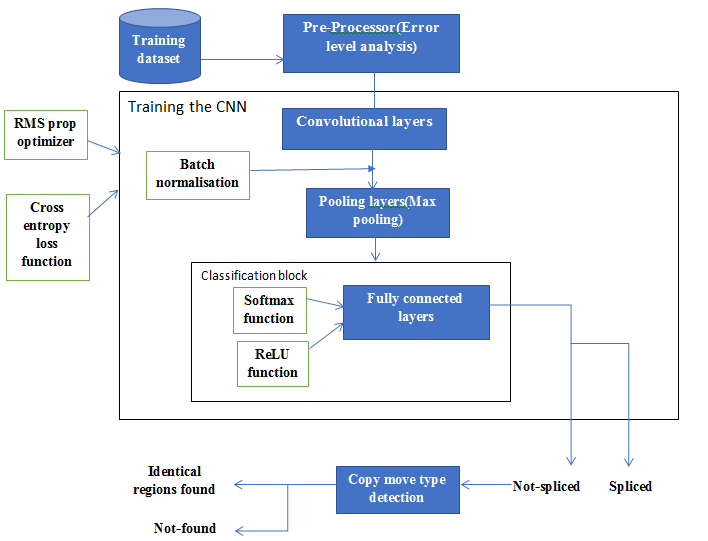
\includegraphics[scale=0.5,width=15cm,height=10cm]{Figures/finalblock.PNG}
\caption{System Architecture showing the entire flow of detecting a forged image}
\label{fig:universe}
\end{figure}

In this architecture the tampered images undergo a certain type of analysis and then it is fed into the neural network for further feature extraction and classification. The training dataset which contains the forged images are analysed for differences in the quality level which might occur due to the editing the image has undergone and resaving it. These comparisons in difference in quality levels within an image is done through the error level analysis and the output of this phase will be given to the CNN.

\tab Each convolutional layer is followed by a normalization process called batch normalization which will increase the accuracy of the CNN model. To give the accurate result the last layer in the classification layer of the neural network uses the softmax activation function which gives the highest activation level. The overall CNN architecture uses RMSprop optimizer which will help the model in converging faster. This will be used to identify the spliced images.
\tab For the detection of copy move forged images a block matching system is used. Where the image is split into blocks and some similarity functions are used to extract if they contain identical regions in the image which will ultimately prove that the image is tampered.

\newpage
\section{CLASS DIAGRAM}
The class diagram of the entire system is shown in figure 4.2. This diagram depicts the functions of various modules in the system clearly. It also shows the interaction between the modules of the system thereby providing a clear idea for implementation.

\begin{figure}[h!]
\centering
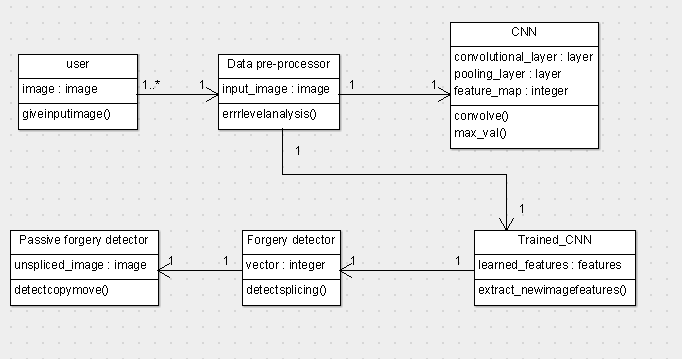
\includegraphics[scale=0.7]{Figures/class.png}
\caption{Class Diagram}
\label{fig:universe}
\end{figure}

